\documentclass[9pt]{article}
\usepackage[letterpaper, margin=2cm]{geometry}
\usepackage[utf8]{inputenc}
\usepackage[sfdefault]{inter}
\usepackage[T1]{fontenc}
\usepackage{amsmath}
\usepackage{graphicx, caption}
\usepackage{xcolor}
\usepackage{subcaption}
\usepackage{siunitx}
\usepackage{booktabs}
\usepackage{tabularx}
\let\temp\rmdefault
\usepackage{fourier}
\let\rmdefault\temp

\usepackage[
  backend=biber,
  style=ieee
]{biblatex}
\addbibresource{spacecraft.bib}

% Title Page
\title{\Huge SARGE\\\Large Final Report}
\author{Jimmy Vaughan\\(101 156 687)}


\begin{document}
\begin{figure}[t]
  \centering
  
\includegraphics[width=.7\linewidth]{CarletonLogo}
\end{figure}
\maketitle
\tableofcontents
\pagenumbering{gobble}
\clearpage
\pagenumbering{arabic}
\section{Introduction}
This preliminary report is intended to inform the reader of the progress made on developing the SARGE satellite.
SARGE stands for \textbf{S}ynthetic~\textbf{A}perture~\textbf{R}adar:~\textbf{G}reenhouse~\textbf{E}missions, a satellite platform designed to monitor for potential leaks of cross-Canada pipelines using synthetic aperture radar.

Good progress has been made towards developing the mass, power, and link budgets of the various subsystems.
Estimations have been made where necessary, and noted, and the development process permits back-filling these determinations with higher quality estimates as they become available.
Preliminary design drawings are available as the last appendix, Appendix~\ref{app:julia}.

\section{Mission Statement}
\subsection{Primary Mission Objectives}
TODO
\subsection{Secondary Mission Objectives}
TODO

\section{Orbit Selection}
The mission requirements state that the primary goal of this mission is to image the entirety of Canada at least every 14~days.
To satisfy this requirement, a geosynchronous orbit with a nonstandard inclination was chosen.
As shown in Figure~\ref{fig:groundtrack}, the ground track of a conical SAR with a minimum elevation angle of \ang{75} covers the entirety of contiguous Canada.

\begin{figure}[hb]
  \centering
  \captionsetup{width=.75\linewidth,font={small},labelfont={bf}}
  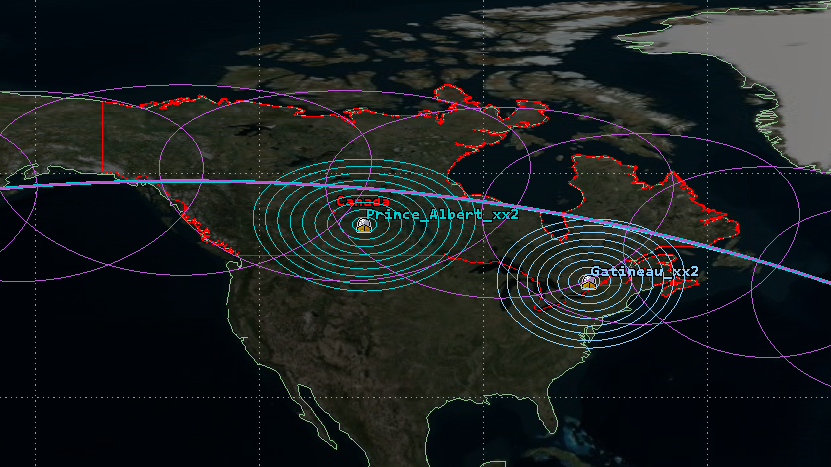
\includegraphics[width=12cm]{groundtrack}
  \caption{Ground swath of SARGE over continental Canada. Ground stations are shown in teal and sky blue, and the majority of Canada is outlined in red ($A\approx\qty{8.342e6}{\square\kilo\metre}$). The magenta circles show the coverage of the SAR beam at some discrete points in time.}
  \label{fig:groundtrack}
\end{figure}

The orbital parameters are summarized in Table~\ref{tab:orbit}.
We can see that the chosen orbit is a circular retrograde orbit with a period of about one sidereal day.
This regularity allows the satellite to image, process, and transmit one~fourteenth of Canada each day, with a consistent and regular ground station access window.

\begin{table}[h]
  \centering
  \captionsetup{width=.75\linewidth,font={small},labelfont={bf}}
    \begin{tabular}{r S|r S}
      \toprule
      \multicolumn{4}{c}{Basic Orbital Parameters}\\
      \midrule
      Period $P$ & \qty{86170.5}{\second} & Arg. of Perigee $\omega$ & \ang{0} \\
      Eccentricity $\epsilon$ & \num{0.0} & LAN $\Omega$ & \ang{50} \\
      Inclinination $i$ & \ang{121} & True Anomaly $\nu$ & \ang{30} \\
      \midrule %\midrule
      \multicolumn{4}{c}{Derived Quantities}\\
      \midrule
      Orbit Radius $r$ & \qty{42166.26}{\kilo\metre} & Orbital Altitude $h$ & \qty{35788.12}{\kilo\metre} \\
      Velocity $v$ & \qty{3.074}{\kilo\metre\per\second} & Orbits per Day $n$ & \qty{1.002663}{\per\day} \\
      \bottomrule
    \end{tabular}
    \caption{Orbital parameters and convenient derived quantities.}
    \label{tab:orbit}
\end{table}

At high altitudes, like GEO, the gravitational forces of the Sun and the Moon become significant, but air drag is generally negligible~\cite{sse}.
The stationkeeping consequences are explored in Appendix~\ref{app:stnkeep}.

\section{Spacecraft Bus}
\subsection{Mass and Power Budget}
According to David Everett of the NASA Goddard Space Flight Center, author of Chapter 14 ``Overview of Spacecraft Design'' in SME-SMAD, the first of the three steps of mass estimation is ``A rough order of magnitude based on payload mass''~\cite[p. 399]{sme}.
Given that sentiment, and the preliminary nature of this report, I feel it is appropriate to base the initial mass estimate on what is described to be data representative of mission type \textit{and} historical data given in Table~14-18~\cite[p. 422]{sme}, as summarized in Table~\ref{tab:mass}, with comments noted in the third column.

\begin{table}[h]
  \centering
  \captionsetup{width=.75\linewidth,font={small},labelfont={bf}}
  %\begin{tabularx}{.8\linewidth}{l|r r X}
  \begin{tabular}{l|r r l}
    \toprule
    Subsystem & Mass\% & Mass & Comments \\
    \midrule
    Payload & \qty{32}{\percent} & \qty{200}{\kilo\gram} & Provided in requirements \\
    Structure \& Mechanisms & \qty{24}{\percent} & \qty{150}{\kilo\gram} & Table~14-18 \\
    Thermal Control & \qty{4}{\percent} & \qty{25.}{\kilo\gram} & ''\\
    Power (incl. harness) & \qty{17}{\percent} & \qty{106}{\kilo\gram}&''\\
    TT\&C & \qty{4}{\percent} & \qty{25}{\kilo\gram}&''\\
    Data Processing & \qty{3}{\percent} & \qty{19}{\kilo\gram}&''\\
    ADCS & \qty{6}{\percent} & \qty{37}{\kilo\gram}&''\\
    Propulsion & \qty{7}{\percent} & \qty{44}{\kilo\gram}&''\\
    Other & \qty{3}{\percent} & \qty{19}{\kilo\gram}&''\\
    \midrule 
    Total Dry Mass & \qty{100}{\percent} & \qty{625}{\kilo\gram} & \\
    Propellant & \qty{72}{\percent} & \qty{450}{\kilo\gram} & May need less (see Appendix~\ref{app:stnkeep})\\
    \midrule 
    Wet Mass & & \qty{1075}{\kilo\gram} & \\
    \bottomrule
  \end{tabular}
  \caption{Preliminary mass budget estimation, based on provided payload mass and the listing for ``High Earth'' in the SME-SMAD~\cite{sme}.}
  \label{tab:mass}
\end{table}


Like the Mass Budget in Table~\ref{tab:mass}, the preliminary power budget below in Table~\ref{tab:power} is based on David~Everett's chapter of the SME-SMAD.
This time, however, a modification to the suggested weights in Table~14-20~\cite[p. 424]{sme}, since no power was allocated to the Structure~\&~Mechanisms subsystem.
As noted in Section~\ref{sec:configuration}, there are several non-oneshot mechanisms on SARGE that will require power.
The payload mass proportion was thus lessened by \qty{2}{\percent}, from \qty{35}{\percent} to \qty{33}{\percent} to give a corresponding mass proportion of \qty{2}{\percent} to the Structures~\&~Mechanisms subsystem.

\begin{table}[h]
  \centering
  \captionsetup{width=.75\linewidth,font={small},labelfont={bf}}
  \begin{tabular}{l|r r l}
    \toprule
    Subsystem & Power\% & Avg. Power & Comments \\
    \midrule
    Payload & \qty{33}{\percent} & \qty{350}{\watt} & Specified in requirements, mod. from Table~14-20 \\ 
    Structure \& Mechanisms & \qty{2}{\percent} & \qty{21}{\watt} & Mod. from Table~14-20 \\
    Thermal & \qty{14}{\percent} & \qty{148}{\watt} & Table~14-20 \\
    Power (incl. harness) & \qty{7}{\percent} & \qty{74}{\watt} & ''\\
    TT\&C & \qty{16}{\percent} & \qty{170}{\watt} & ''\\
    Data Processing & \qty{10}{\percent} & \qty{106}{\watt} &''\\
    ADCS & \qty{16}{\percent} & \qty{170}{\watt}&''\\
    Propulstion & \qty{2}{\percent} & \qty{21}{\watt} & ''\\
    \midrule
    Total & \qty{100}{\percent} & \qty{1061}{\watt} &\\
    \bottomrule
  \end{tabular}
  \caption{Preliminary power budget estimation, based on provided payload mass and the listing for ``High Earth'' in the SME-SMAD~\cite{sme}, modified to allow for powered mechanisms.}
  \label{tab:power}
\end{table}

\subsection{Configuration}
The configuration of SARGE is a nadir-pointing 3-axis stabilized solar-powered satellite.
An annotated isometric view of the preliminary design/layout is shown in Figure~\ref{fig:iso}.

\begin{figure}[h]
  \centering
  \captionsetup{width=.75\linewidth,font=small,labelfont=bf}
  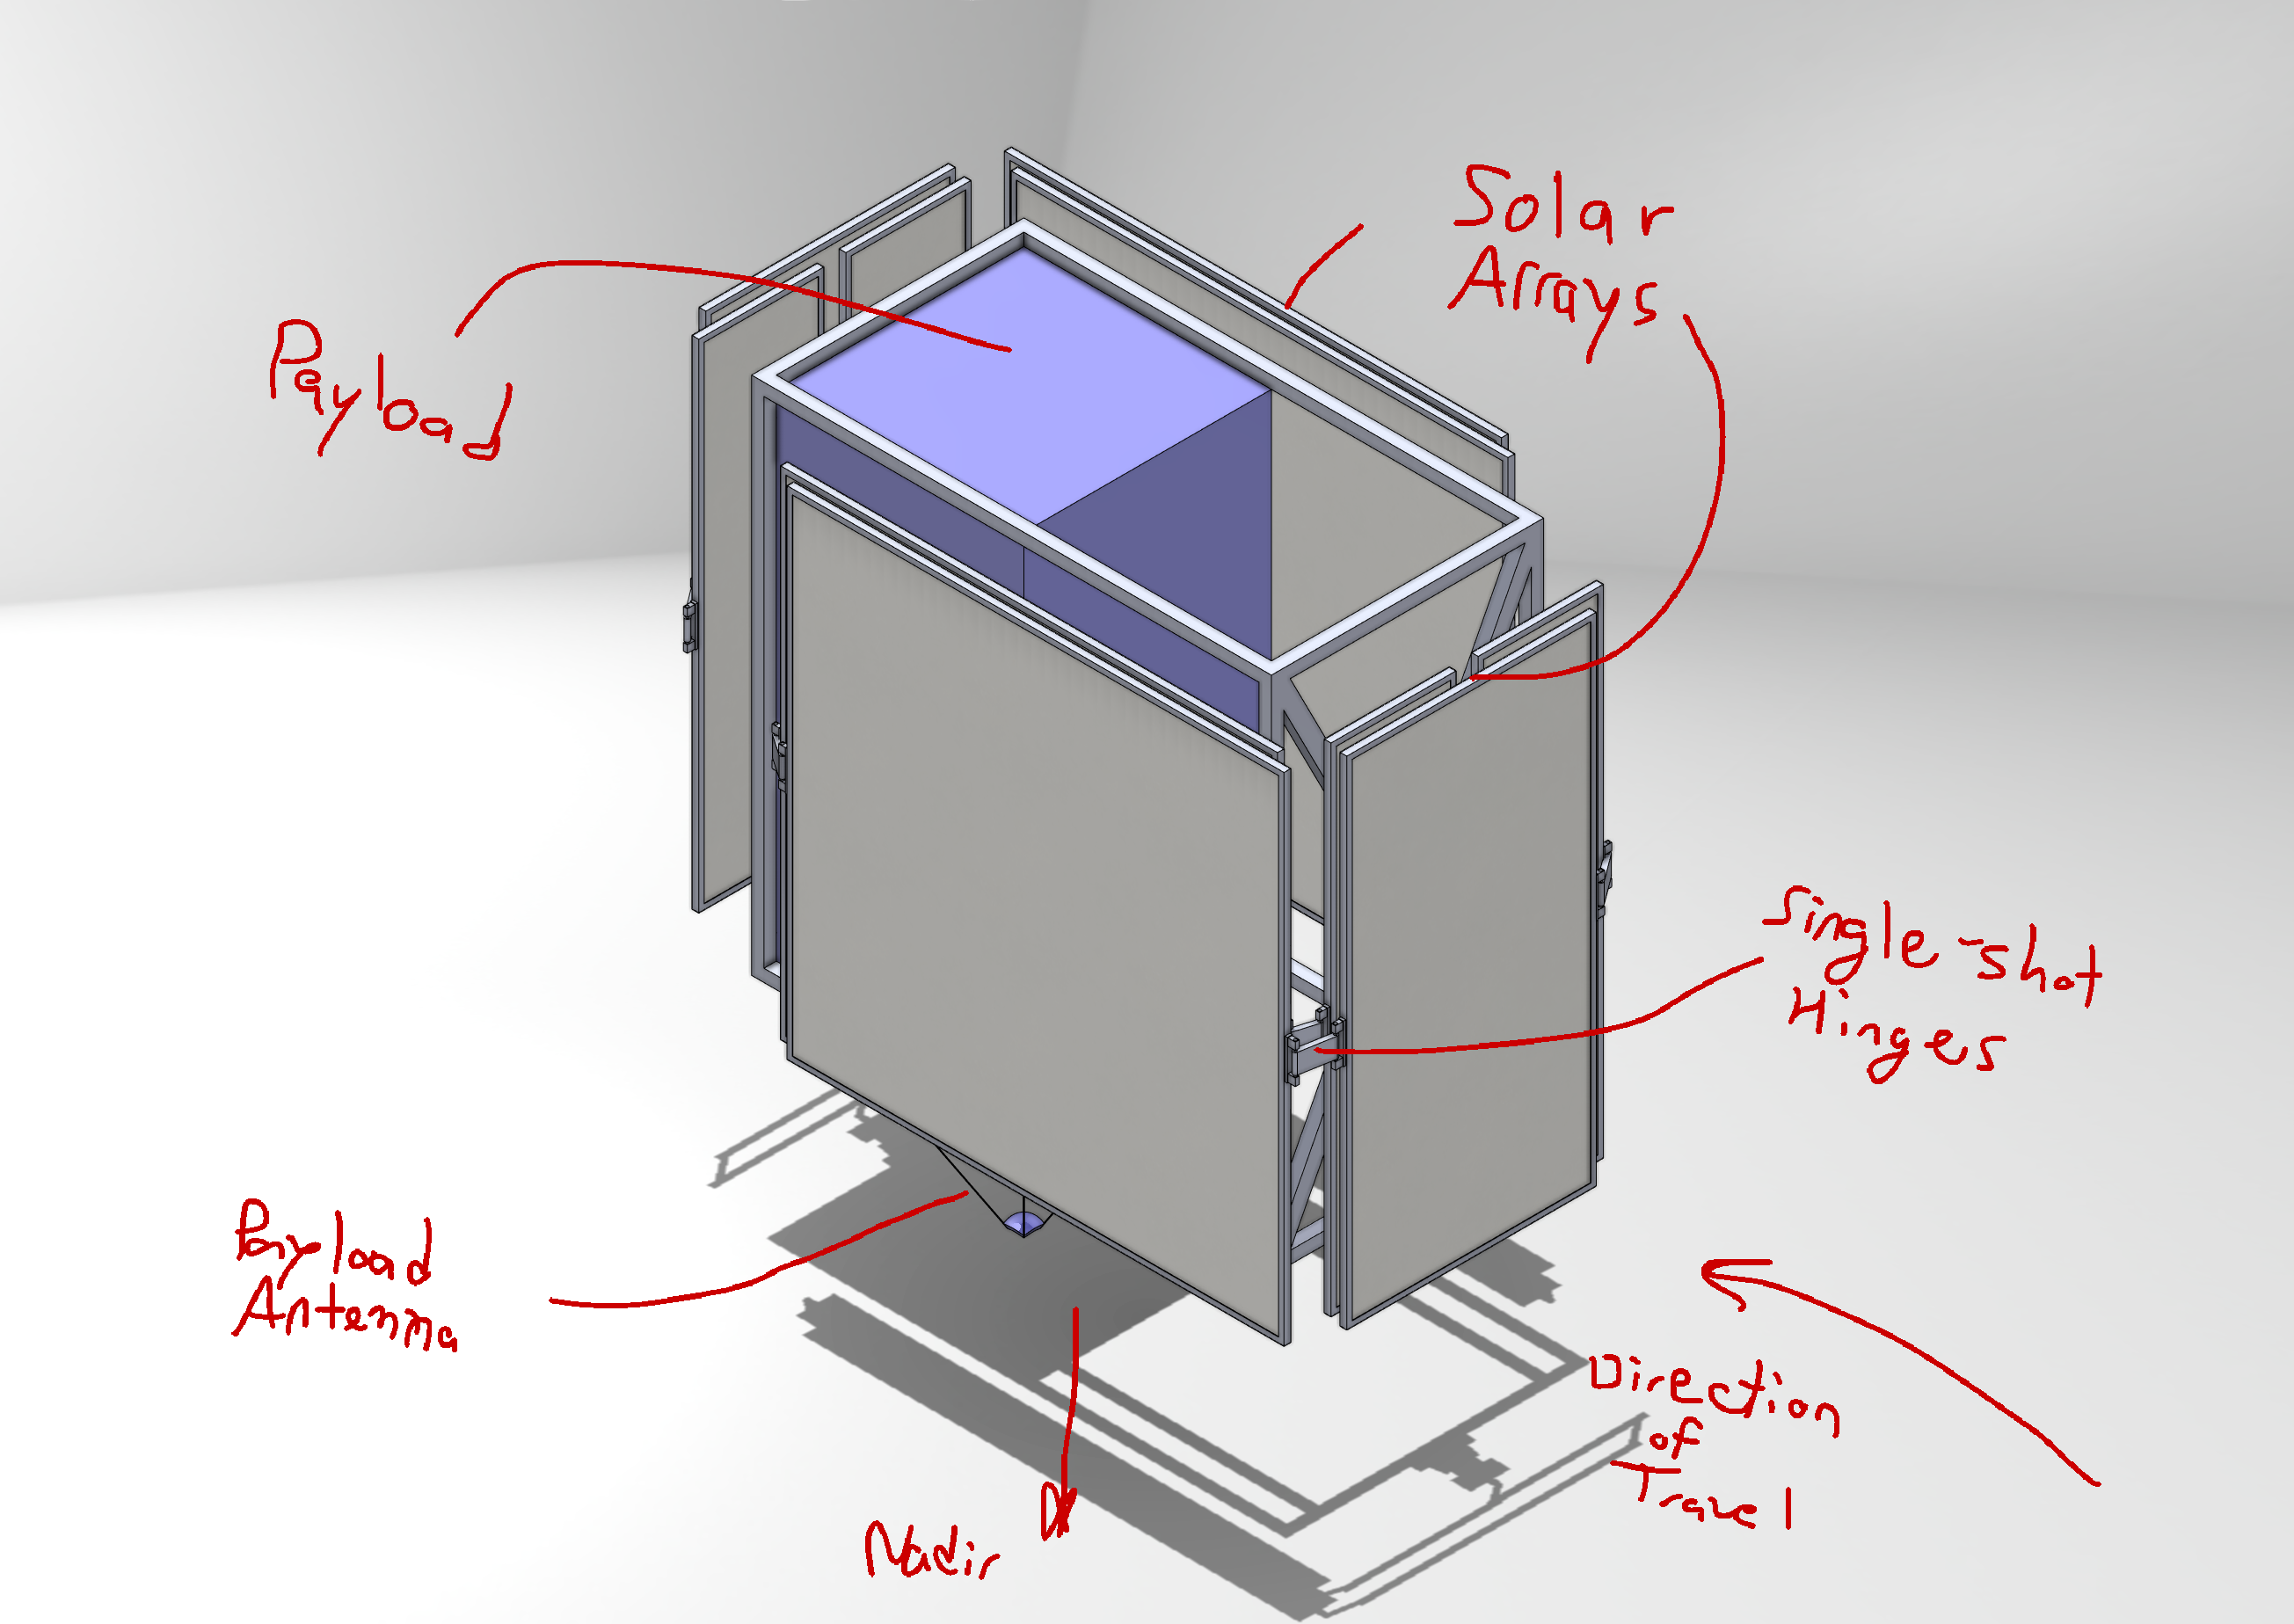
\includegraphics[width=.4\linewidth]{iso}
  \caption{Isometric view of the satellite with annotation in red to aid understanding.}
  \label{fig:iso}
\end{figure}

As can hopefully be seen, the major components currently include 2 solar arrays, articulated only for launching, via single-shot hinges at each meeting point.
These arrays are gimbaled in one axis, shown in the front view, Figure~\ref{fig:front}.
The direction of travel is shown in Figure~\ref{fig:iso}, as well as the nadir pointing direction.

\begin{figure}[h]
  \centering
  \captionsetup{width=.75\linewidth,font=small,labelfont=bf}
  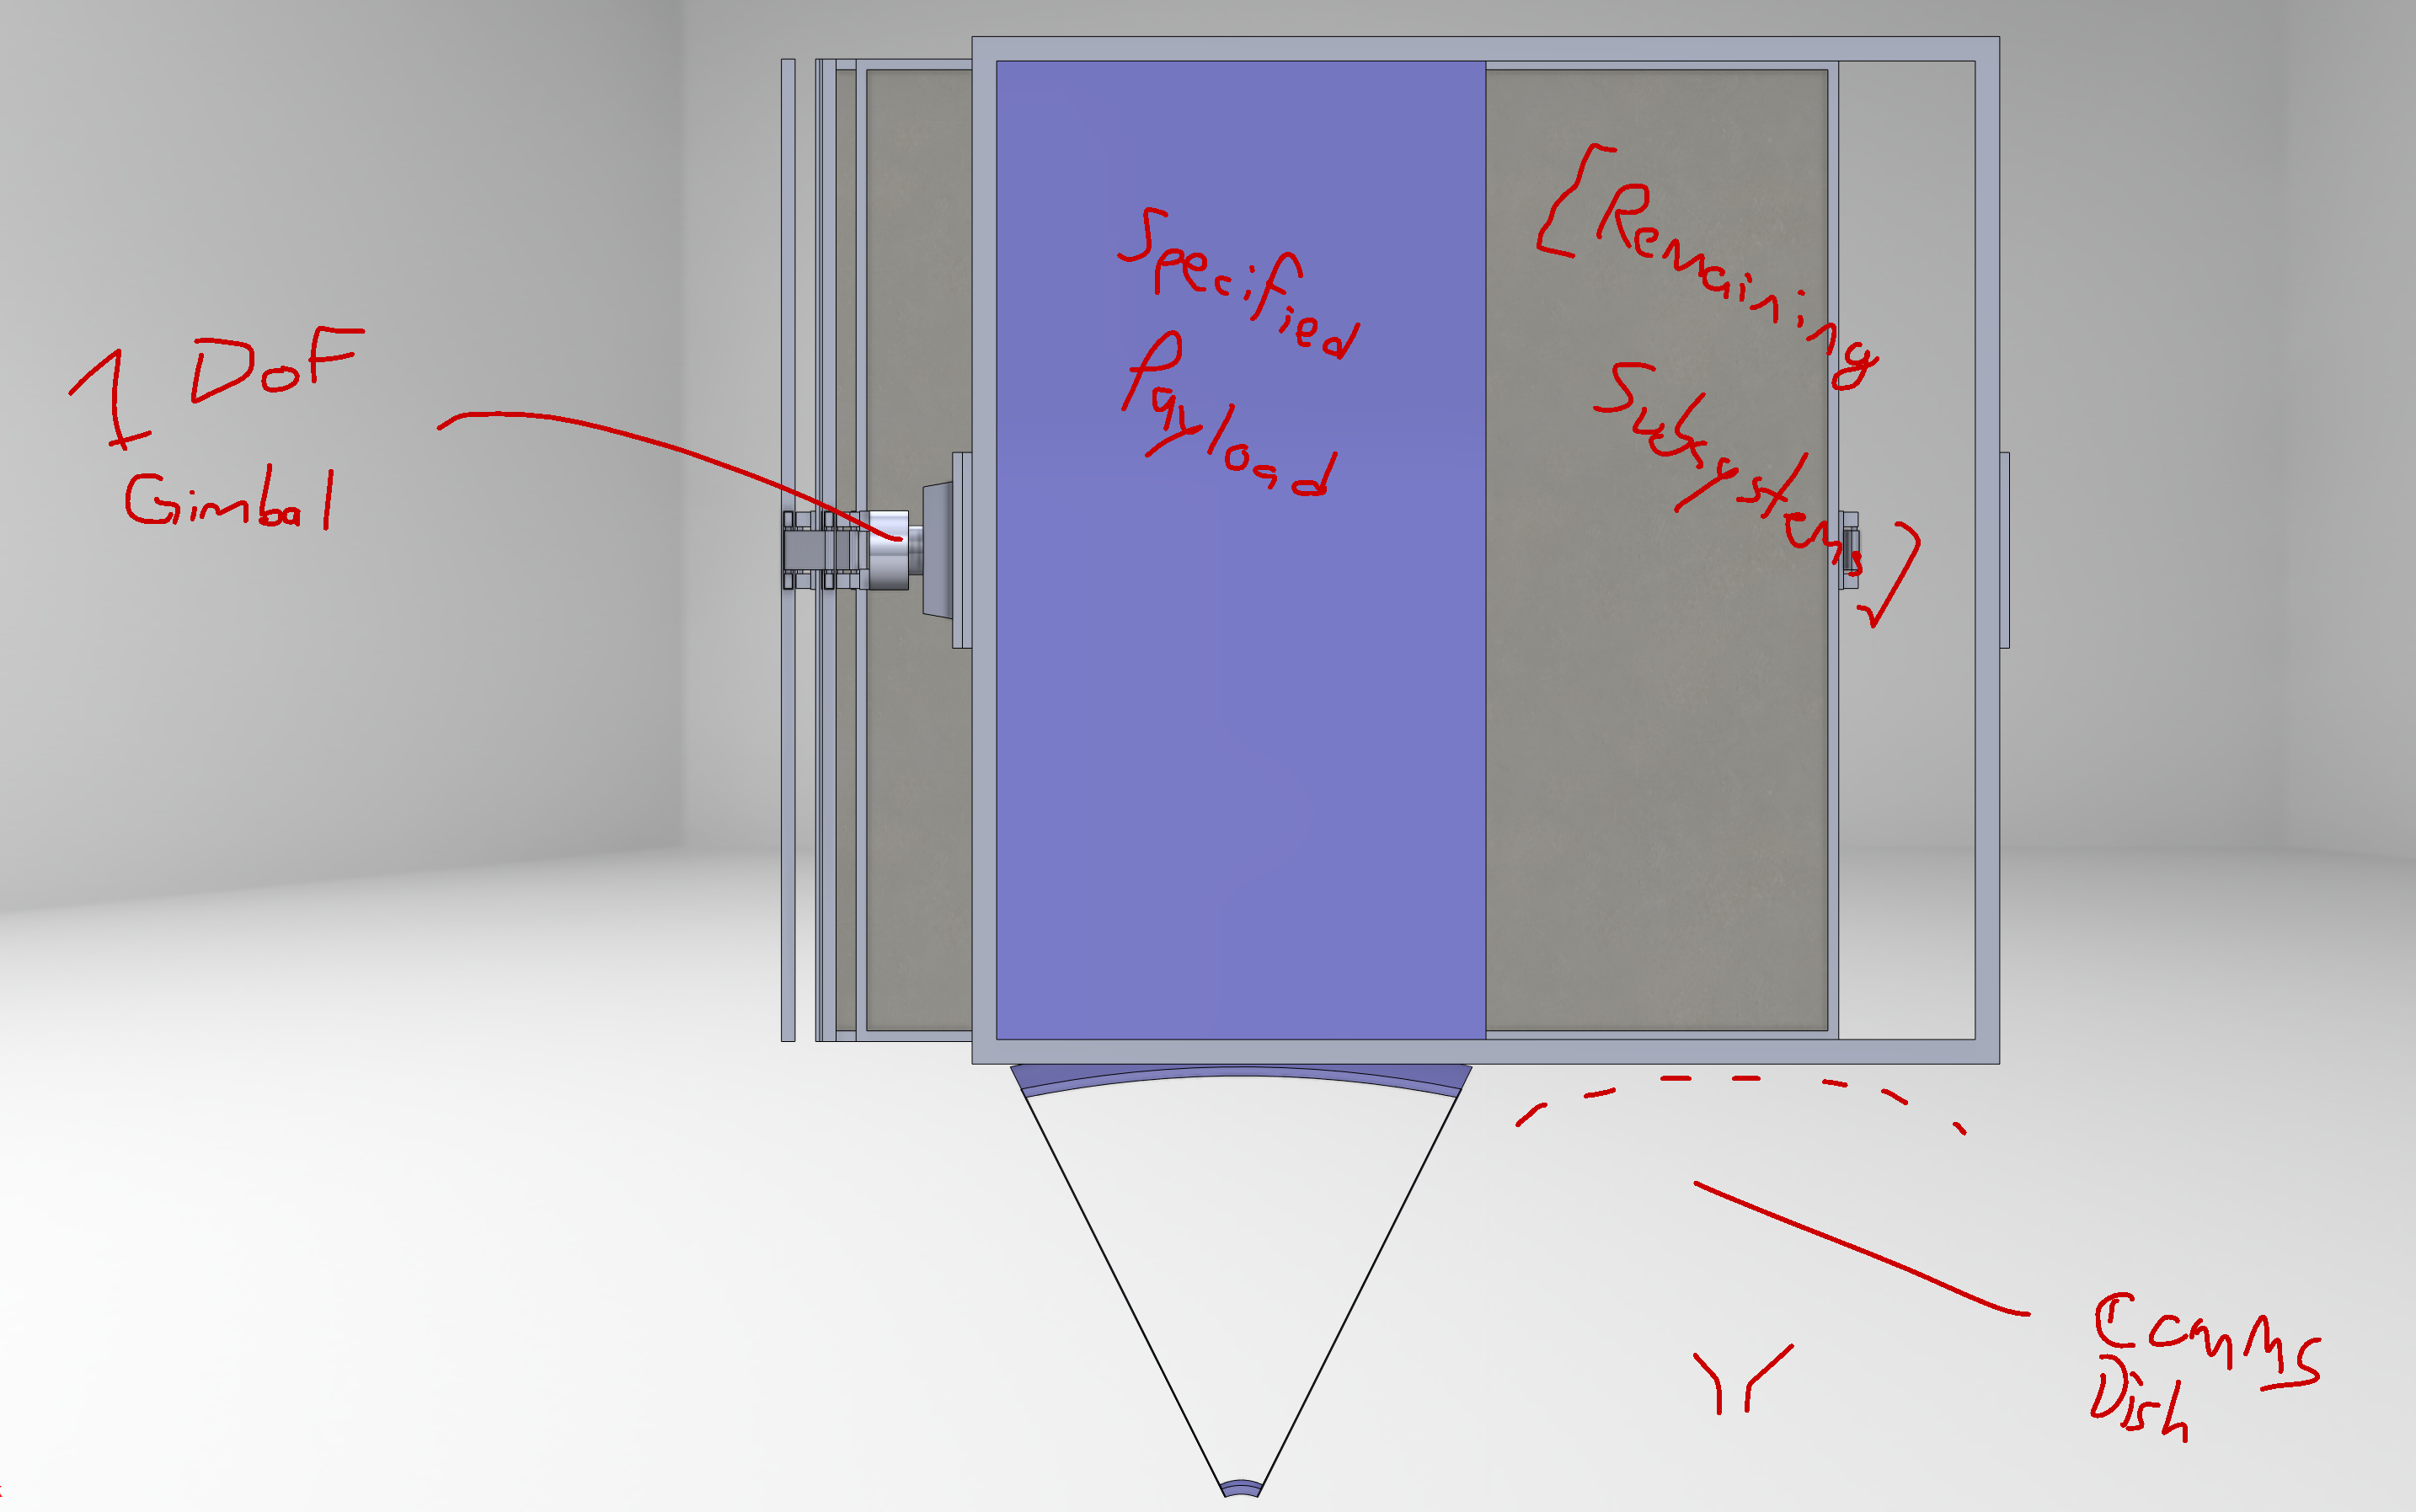
\includegraphics[width=.4\linewidth]{front}
  \caption{Front view of SARGE with annotation in red. One of the solar panel arrays is hidden so as not to obstruct the interior of the frame.}
  \label{fig:front}
\end{figure}

Since the masses of the solar arrays are identical, and they are symmetric about the nadir axis, and since the mass proportion of the payload is only around \qty{32}{\percent} of the total dry mass, the remaining subsystems should make it so that the center of mass is not located within the payload container.
This means that an ADCS system with reaction wheels should be able to be located directly in line with all three axes relative to the center of inertia, so pointing should be easily controllable.
The remaining subsystems will all ideally fit in the remaining payload-sized area to the right of the payload in Figure~\ref{fig:front}.

More engineering drawings are available in Appendix~\ref{app:julia}.


\subsection{Preliminary Design of Spacecraft Subsystems}


\subsubsection{Communications Subsystem}
Based on both slide deck 6, ``TTC'', and select portions of the SME-SMAD, the uplink and downlink link budgets are summarized in Table~\ref{tab:link}.
As well, the downlink and uplink frequencies were chosen according to Professor~Jim~Wight's course handout for ELEC~4509.
It's noted in that handout that frequency ranges 7.25-7.30~GHz and 7.975-8.025~GHz are reserved for downlink and uplink satellite communications, respectively~\cite[II, p. 3]{commlinks}.
\begin{table}[h]
  \centering
  \captionsetup{width=.75\linewidth,font=small,labelfont=bf}
  \begin{tabular}{c|rl|l}
    \toprule
    Uplink & Value & Unit & Comments \\
    \midrule
    $P_t$ & \num{23.01} & \si{\decibel\watt} & \qty{200}{\watt} ground transmitter assumed\\
    $G_t$ & \num{57.74} & \si{\decibel} & Eq.~\ref{eq:200}\\
    $L_\text{path}$ & \num{202.68} & \si{\decibel} & Eq.~\ref{eq:203}\\
    $L_\text{point}$ & \num{18.42} & \si{\decibel} & Eq.~\ref{eq:303}\\
    $L_\text{atmosphere}$ & \num{10.00} & \si{\decibel} & Assumed\\
    $k$ & \num{-228.60} & \si{\decibel\joule\per\kelvin} & \\
    $B$ & \num{37.00} & \si{\decibel\hertz} & Eq.~\ref{eq:201}\\
    $G_r$ & \num{28.61} & \si{\decibel} & Eq.~\ref{eq:100}\\
    $T$ & \num{27.00} & \si{\decibel\kelvin} & Assumed\\
    \midrule
    ${C/N}_\text{achieved}$ & \num{55.54} & \si{\decibel} & Eq.~\ref{eq:uplinkachieved}\\
    ${C/N}_\text{required}$ & \num{8.16} & \si{\decibel} & Eq.~\ref{eq:202}\\
    \midrule
    Margin & \num{47.39} & \si{\decibel}& \\
    \bottomrule \toprule
    Downlink & Value & Unit & Comments\\
    $P_t$ & \num{20.00} & \si{\decibel\watt} & \qty{100}{\watt} of \qty{170}{\watt} estimated in power budget\\
    $G_t$ & \num{28.61} & \si{\decibel} & Eq.~\ref{eq:100}\\
    $L_\text{path}$ & \num{201.85} & \si{\decibel} & Eq.~\ref{eq:101}\\
    $L_\text{point}$ & \num{0.36} & \si{\decibel} & Eq.~\ref{eq:302}\\
    $L_\text{atmosphere}$ & \num{10.00} & \si{\decibel} & Assumed\\
    $k$ & \num{-228.60} & \si{\decibel\joule\per\kelvin} & \\
    $B$ & \num{70.77} & \si{\decibel\hertz} & Eq.~\ref{eq:downlinkbw}\\
    $G/T$ & \num{46.94} & \si{\decibel\per\kelvin} & Eq.~\ref{eq:minGT}\\
    \midrule
    ${C/N}_\text{achieved}$ & \num{41.17} & \si{\decibel} & Eq.~\ref{eq:downlinkachieved}\\
    ${C/N}_\text{required}$ & \num{11.52} & \si{\decibel} & Eq.~\ref{eq:102}\\
    \midrule
    Margin & \num{29.65} & \si{\decibel} & \\
    \bottomrule
  \end{tabular}
  \caption{Preliminary link budget, based on noted assumptions and analyses detailed in Appendix~\ref{app:linkbudget}.}
  \label{tab:link}
\end{table}

The uplink ${C/N}_\text{achieved}$ was calculated using the following expression, where square brackets indicate logarithmic quantities:
\begin{equation}\label{eq:uplinkachieved}
  [C/N]_\text{achieved}=[P_t] + [G_t] + [G_r] - [L_\text{path}] - [L_\text{point}] - [L_\text{atmosphere}] - [k] -[T]-[B]
\end{equation}
Whereas the downlink ${C/N}_\text{achieved}$ was calculated using a slightly different methodology, where the minimum certifiable $G/T$ figure is found by~\cite[I, p. 40]{commlinks}:
\begin{equation}\label{eq:minGT}
  \frac GT\ge \qty{40.7}{\decibel}+20\log{\frac f4}
\end{equation}
where $G/T$ is in \si{\decibel\per\kelvin}, and $f$ is in \si{\giga\hertz}.
Since that's the minimum figure of merit to be certified for a ground station, I took that as the figure of merit for Gatineau.
Then,
\begin{equation}\label{eq:downlinkachieved}
  [{C/N}]_\text{achieved}=[P_t]+[G_t]+\left[\frac GT\right]-[L_\text{path}]-[L_\text{point}]-[L_\text{atmosphere}]-[k]-[B]
\end{equation}

\subsubsection{Power Subsystem}
TODO
\subsubsection{Attitude Determination and Control Subsystem}
TODO
\subsubsection{Propulsion Subsystem}

Given the GTO... stationkeeping... disposal...

Can't use ion engine because of power requirements...\cite{next}

yeah
\subsubsection{etc...}


\section{Launcher Selection Trade Study}
A selection of launch platforms still in use as of 2025 were considered, with the key parameters summarized in Table~\ref{tab:launchertrade}.
All launchers deliver their payload to GTO, with fairly minor differences in delivered transfer orbit, with the exception of the Ariane~62.

\begin{table}[h]
  \centering
  \captionsetup{width=.75\linewidth,font=small,labelfont=bf}
  \begin{tabular}{lc|cccc|ccr}
    \toprule
    Platform & Country & $i$ (\si{\degree}) & $h_p$ (\si{\kilo\meter}) & $h_a$ (\si{\kilo\meter}) & $\omega_p$ (\si{\degree}) & $M$ (\si{\kilo\gram}) & $D$ (\si{\meter}) & Cost \\
    \midrule
    SpaceX Falcon 9~\cite{spacex} & USA & \num{28.5} & \num{185} & \num{35788} & \num{0} & \num{5800}\textdagger & \num{3.7} & \num{69.75}~\cite{spacexprice} \\
    Ariane~62~\cite{ariane} & France & \num{6} & \num{250} & \num{35786} & \num{178} & \num{4500} & \num{5.4} & \num{88}\hspace{1.55em}\cite{arianeprice}\\
    Atlas V 401~\cite{atlasv} & USA & \num{27} & \num{185} & \num{35786} & \num{180} & \num{4750} & \num{4.0} & \num{109}\hspace{.6em} \cite{atlasvprice}\\
    Long March 3B~\cite{longmarch} & China & \num{28.5} & \num{200} & \num{35786} & \num{178} & \num{5100} & \num{4.0} & \num{70}\hspace{.9em}\cite{longmarchprice}\\
    \bottomrule
  \end{tabular}
  \caption{Selected launch platform comparison. \textdagger: includes payload adapter. Prices in millions USD, not adjusted for inflation.}
  \label{tab:launchertrade}
\end{table}



\section{Conclusions}
Although further analysis is required to ensure that the current configuration can reject/retain enough heat, and the delta V budget is yet to be done, the current iteration of SARGE looks to be reasonable.
The mass distribution and total mass falls within the ranges typical of a GEO mission.
The total estimated power draw is somewhat lower than what is mentioned in the course slides.
The link budget has good margins, even after adding an assumed atmospheric loss.



\clearpage
\appendix

\printbibliography
\clearpage
\section{Orbital Perturbations and $\Delta V$}\label{app:orbpert}

SME-SMAD equations (9-46) and (9-47) on pg.~219 give approximate worse case $\Delta V$ relations per year~\cite{sme}:
\begin{align}
  {\Delta V}_\text{Moon} &= 102.67\cos\alpha\sin\alpha\hspace{2em}\text{(m/s per year)}\\
  {\Delta V}_\text{Sun} &= 40.17\cos\gamma\sin\gamma\hspace{2.7em}\text{(m/s per year)}
\end{align}
where $\alpha$ is the angle between the orbit plane and the Moon's orbit, and $\gamma$ is the angle between the orbit plane and the ecliptic.

\subsection{Stationkeeping}\label{app:stnkeep}
The angles estimated in Appendix~\ref{app:orbplanes} and illustrated in Figure~\ref{fig:moonorbit}, substituted into the preceding expressions, yield:
\begin{equation}
  {\Delta V}_\text{Moon} = 102.67\cos{\ang{92.42}}\sin{\ang{92.42}} = \qty{4.331}{\meter\per\second\per yr}
\end{equation}
\begin{equation}
  {\Delta V}_\text{Sun} = 40.17\cos{\ang{97.56}}\sin{\ang{92.42}} = \qty{5.239}{\meter\per\second\per yr}  
\end{equation}
And then, for the design lifetime of 5 years, the total $\Delta V$ for North-South stationkeeping is the product of the sum of the above:
\begin{equation}
  {\Delta V}_{NS} = ({\Delta V}_\text{Moon} + {\Delta V}_\text{Sun}) \times \qty{5}{yr} = \qty{47.85}{\meter\per\second}
\end{equation}
This is significantly less than the example value of about \qty{51.48}{\meter\per\second\per yr} given in the SME-SMAD for a GEO orbit with an inclination $i$ of \ang{0}~\cite{sme}.
This makes sense, since for a equatorial GEO orbit the Ecliptic and Lunar planes would be between \ang{23.44} and \ang{28.68}, whereas SARGE's highly inclined orbital plane is at nearly right angles to the Ecliptic and Lunar planes, somewhat balancing the perturbing forces of both.

The transverse (East-West) stationkeeping requirement is mentioned as about \qty{10}{\percent} of the North-South stationkeeping requirements~\cite{sme}, however I believe that the high inclination of SARGE will work against us in this scenario, as the oblateness of Earth around the equator will have a more pronounced effect for orbits that do not closely follow the equator.
As well, this oblateness likely has an effect on the North-South stationkeeping, since we're dealing with neither a polar nor equatorial orbit.
For this reason, I'm going to estimate the East-West stationkeeping to be equal to the North-South:
\begin{equation}
  {\Delta V}_{EW} = {\Delta V}_{NS} = \qty{47.85}{\meter\per\second}%pg 219
\end{equation}
This ought to roughly account for the stationkeeping requirements of the spacecraft at this stage of design. 

\subsection{Decommissioning}

The SME-SMAD recommends handling the special scarcity and properties of the GEO orbit (specifically its vulnerability to debris and junk) by raising spacecraft \qty{500}{\kilo\metre} above GEO at the end of their life.
The $\Delta V$ required for that is
\begin{equation}
  {\Delta V}_\text{disposal} = \qty{18}{\metre\per\second}
\end{equation}
from SME-SMAD page 233 for decommissioning a GEO satellite~\cite{sme}, and the propellant mass will be found at a later date after an in-depth $\Delta V$ analysis.

\subsection{Orbital Transfer}
The transfer from the SpaceX GTO orbit in Table~\ref{tab:launchertrade} will be a combined plane-change and elliptical-to-circular maneuver.
The $\Delta V$ required for such a change is~\cite{aero3240}:
\begin{equation}
  \Delta V=\sqrt{v_1^2+v_2^2-2v_1v_2\cos{\Delta i}}
\end{equation}
where $\Delta i=\ang{121}-\ang{28.5}=\ang{92.5}$, and $v_1,\,v_2$ are the orbital velocities of the transfer orbit and final orbit respectively.
The full calculation is scanned and attached before the preliminary drawings of Appendix~\ref{app:julia}.
Hand calculations were chosen as a change of pace.
The final result is a $\Delta V$ of \qty{3.5253}{\kilo\meter\per\second}.


\section{Power and Configuration Implications}\label{app:powerandconf}
\subsection{Power Collection and Storage}\label{app:powercollection}
Given the estimated total average power presented in Table~\ref{tab:power}, \qty{1061}{\watt}, the required solar panel coverage can be estimated following the example in slide deck 7, ``Power'', where the following expression is provided on slide~17:
\begin{equation}
  {PD}_\text{out}={PD}_\text{in}\eta\cos\theta
\end{equation}
where ${PD}_\text{out/in}$ is the power density of out of and into the solar array in \si{\watt\per\meter\squared}, $\eta$ is the power conversion efficiency of the cells, and $\theta$ is the solar incident angle.
Taking the incident solar power as \qty{1366}{\watt\per\meter\squared}, and the achieved efficiency of GaAs cells provided in slide~18 of \qty{18.5}{\percent}, with a worst-case incident angle of about \ang{10} (since the angle of the orbital plane to the ecliptic is \ang{97.56}, found in Appendix~\ref{app:orbplanes}), then
\begin{equation}
  {PD}_\text{out}=\qty{1366}{\watt\per\meter\squared}\cdot\qty{18.5}{\percent}\cdot\cos(\ang{10})= \qty{248.87}{\watt\per\meter\squared}
\end{equation}
Then, dividing the total average power required by the spacecraft (and noting that the spacecraft spends no time in eclipse), the minimum required illuminated area of the solar array is
\begin{equation}
  A_\text{solar,min} = \frac{P_\text{total}}{PD_\text{out}} = \qty{4.26}{\square\meter}
\end{equation}
Since the spacecraft is orbiting in a plane nearly perpendicular to the ecliptic plane, a 1~DoF mechanism for the pointing of the solar array with an angular envelope of $\pm\ang{10}$ should be sufficient to ensure optimal solar collection.
This fact and the lack of eclipse time is well conveyed by Figure~\ref{fig:eclipse} below, showing no part of the orbital track lying in eclipse.

\begin{figure}[h]
  \centering
  \captionsetup{width=.75\linewidth,font=small,labelfont=bf}
  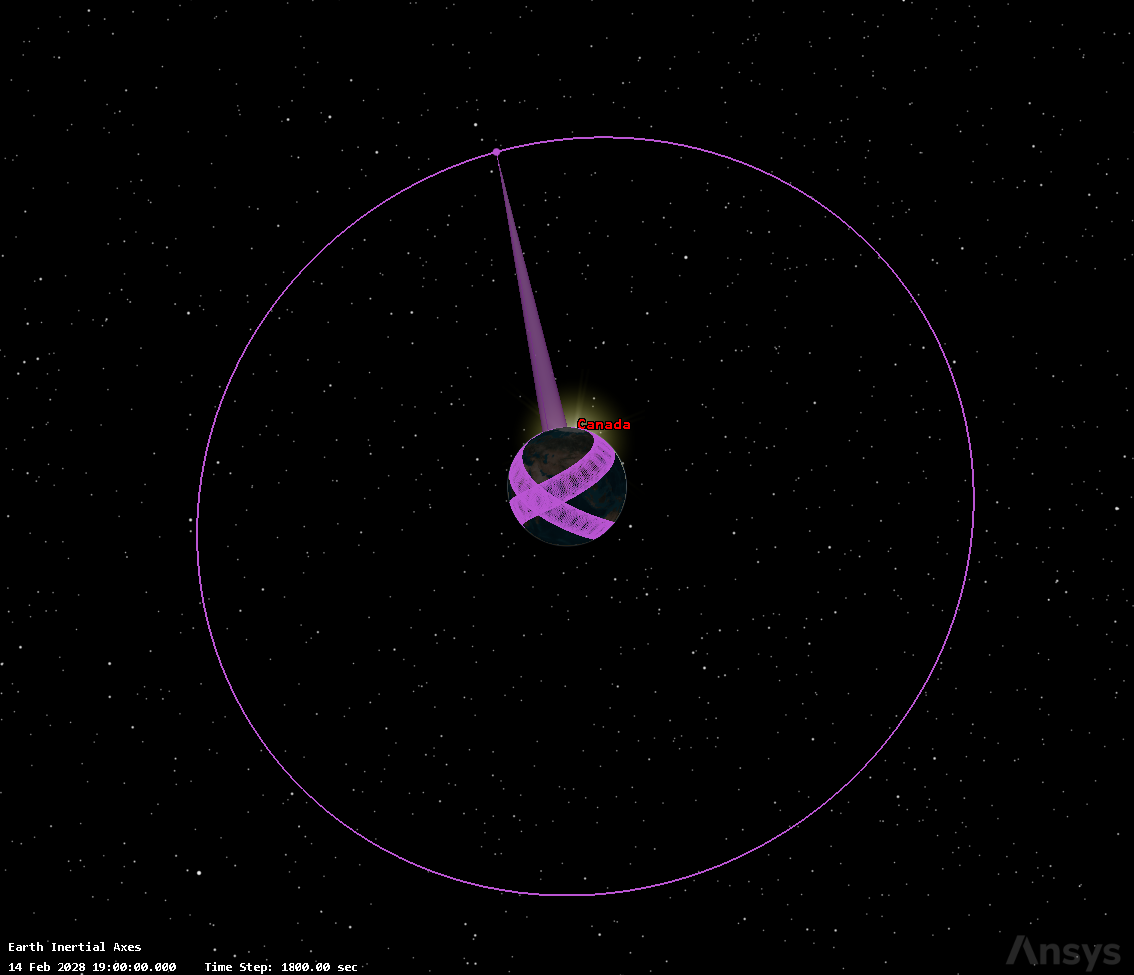
\includegraphics[width=8cm]{zeroeclipse}
  \caption{Demonstration of zero eclipse time via STK 3D view. The sun is visible just over the horizon.}
  \label{fig:eclipse}
\end{figure}

\subsection{Configuration Choices}
In order to accomodate the necessary surface area of the solar panels in a compact way with margins to account for structural frames that would block cells of the solar array, and to pre-emptively take into account the packing of the spacecraft into a launch platform, a quick sketch (Figure~\ref{fig:solarsketch}) showed that the structure should follow roughly a form factor of $\SI{1}{\meter}\times\SI{1}{\meter}\times\SI{0.5}{\meter}$.
This allows the compact packing of nominally \SI{6}{\square\meter} of solar panels, which well exceeds the required \SI{4.26}{\square\meter}.
In later analysis, it will be shown how much of a margin we have to block that area with support structures when EOL conditions and degradation is taken into account.

Table~21-5 in the SME-SMAD notes that travelling wave tube amplifiers (TWTA)s are about 50-60\% efficient for X-band and weigh about \qty{2.5}{\kilo\gram} including power converter~\cite[p. 637]{sme}.
Table~16-16 in the SME-SMAD notes that parabolic reflectors weigh between 10-30~kg~\cite[p. 484]{sme}.

\clearpage
\section{Fun!}
This section is named ``Fun!'' unironically -- these were fun.

\subsection{Fun Annulus Geometry}\label{app:annulus}
To approximate the arc angle subtended by the \ang{10} elevation $\delta$ access requirement, I created a quick sketch shown in Figure~\ref{fig:annulus} to wrap my head around the geometry.
I then used the formula for worst-case distance $d$ from slide deck 6 to find the corresponding half angle $\gamma$:
\begin{equation}
  d=R_\text{Earth}\left(
    \sqrt{\left(\frac{r}{R_\text{Earth}}\right)^2-\cos^2\delta}
    -\sin\delta
  \right)
\end{equation}
From my sketch,
\begin{equation}
  \gamma = \sin^{-1}\left(\frac{d\sin(\ang{90}+\delta)}{r}\right)
\end{equation}
And thus the access ratio is the ratio between the access arc and the total arc (circumference):
\begin{equation}
  \text{Access Ratio} = \frac{2\gamma r}{2\pi r} = \qty{39.69}{\percent}
\end{equation}

\begin{figure}[h]
  \centering
  \captionsetup{width=.75\linewidth,font=small,labelfont=bf}
  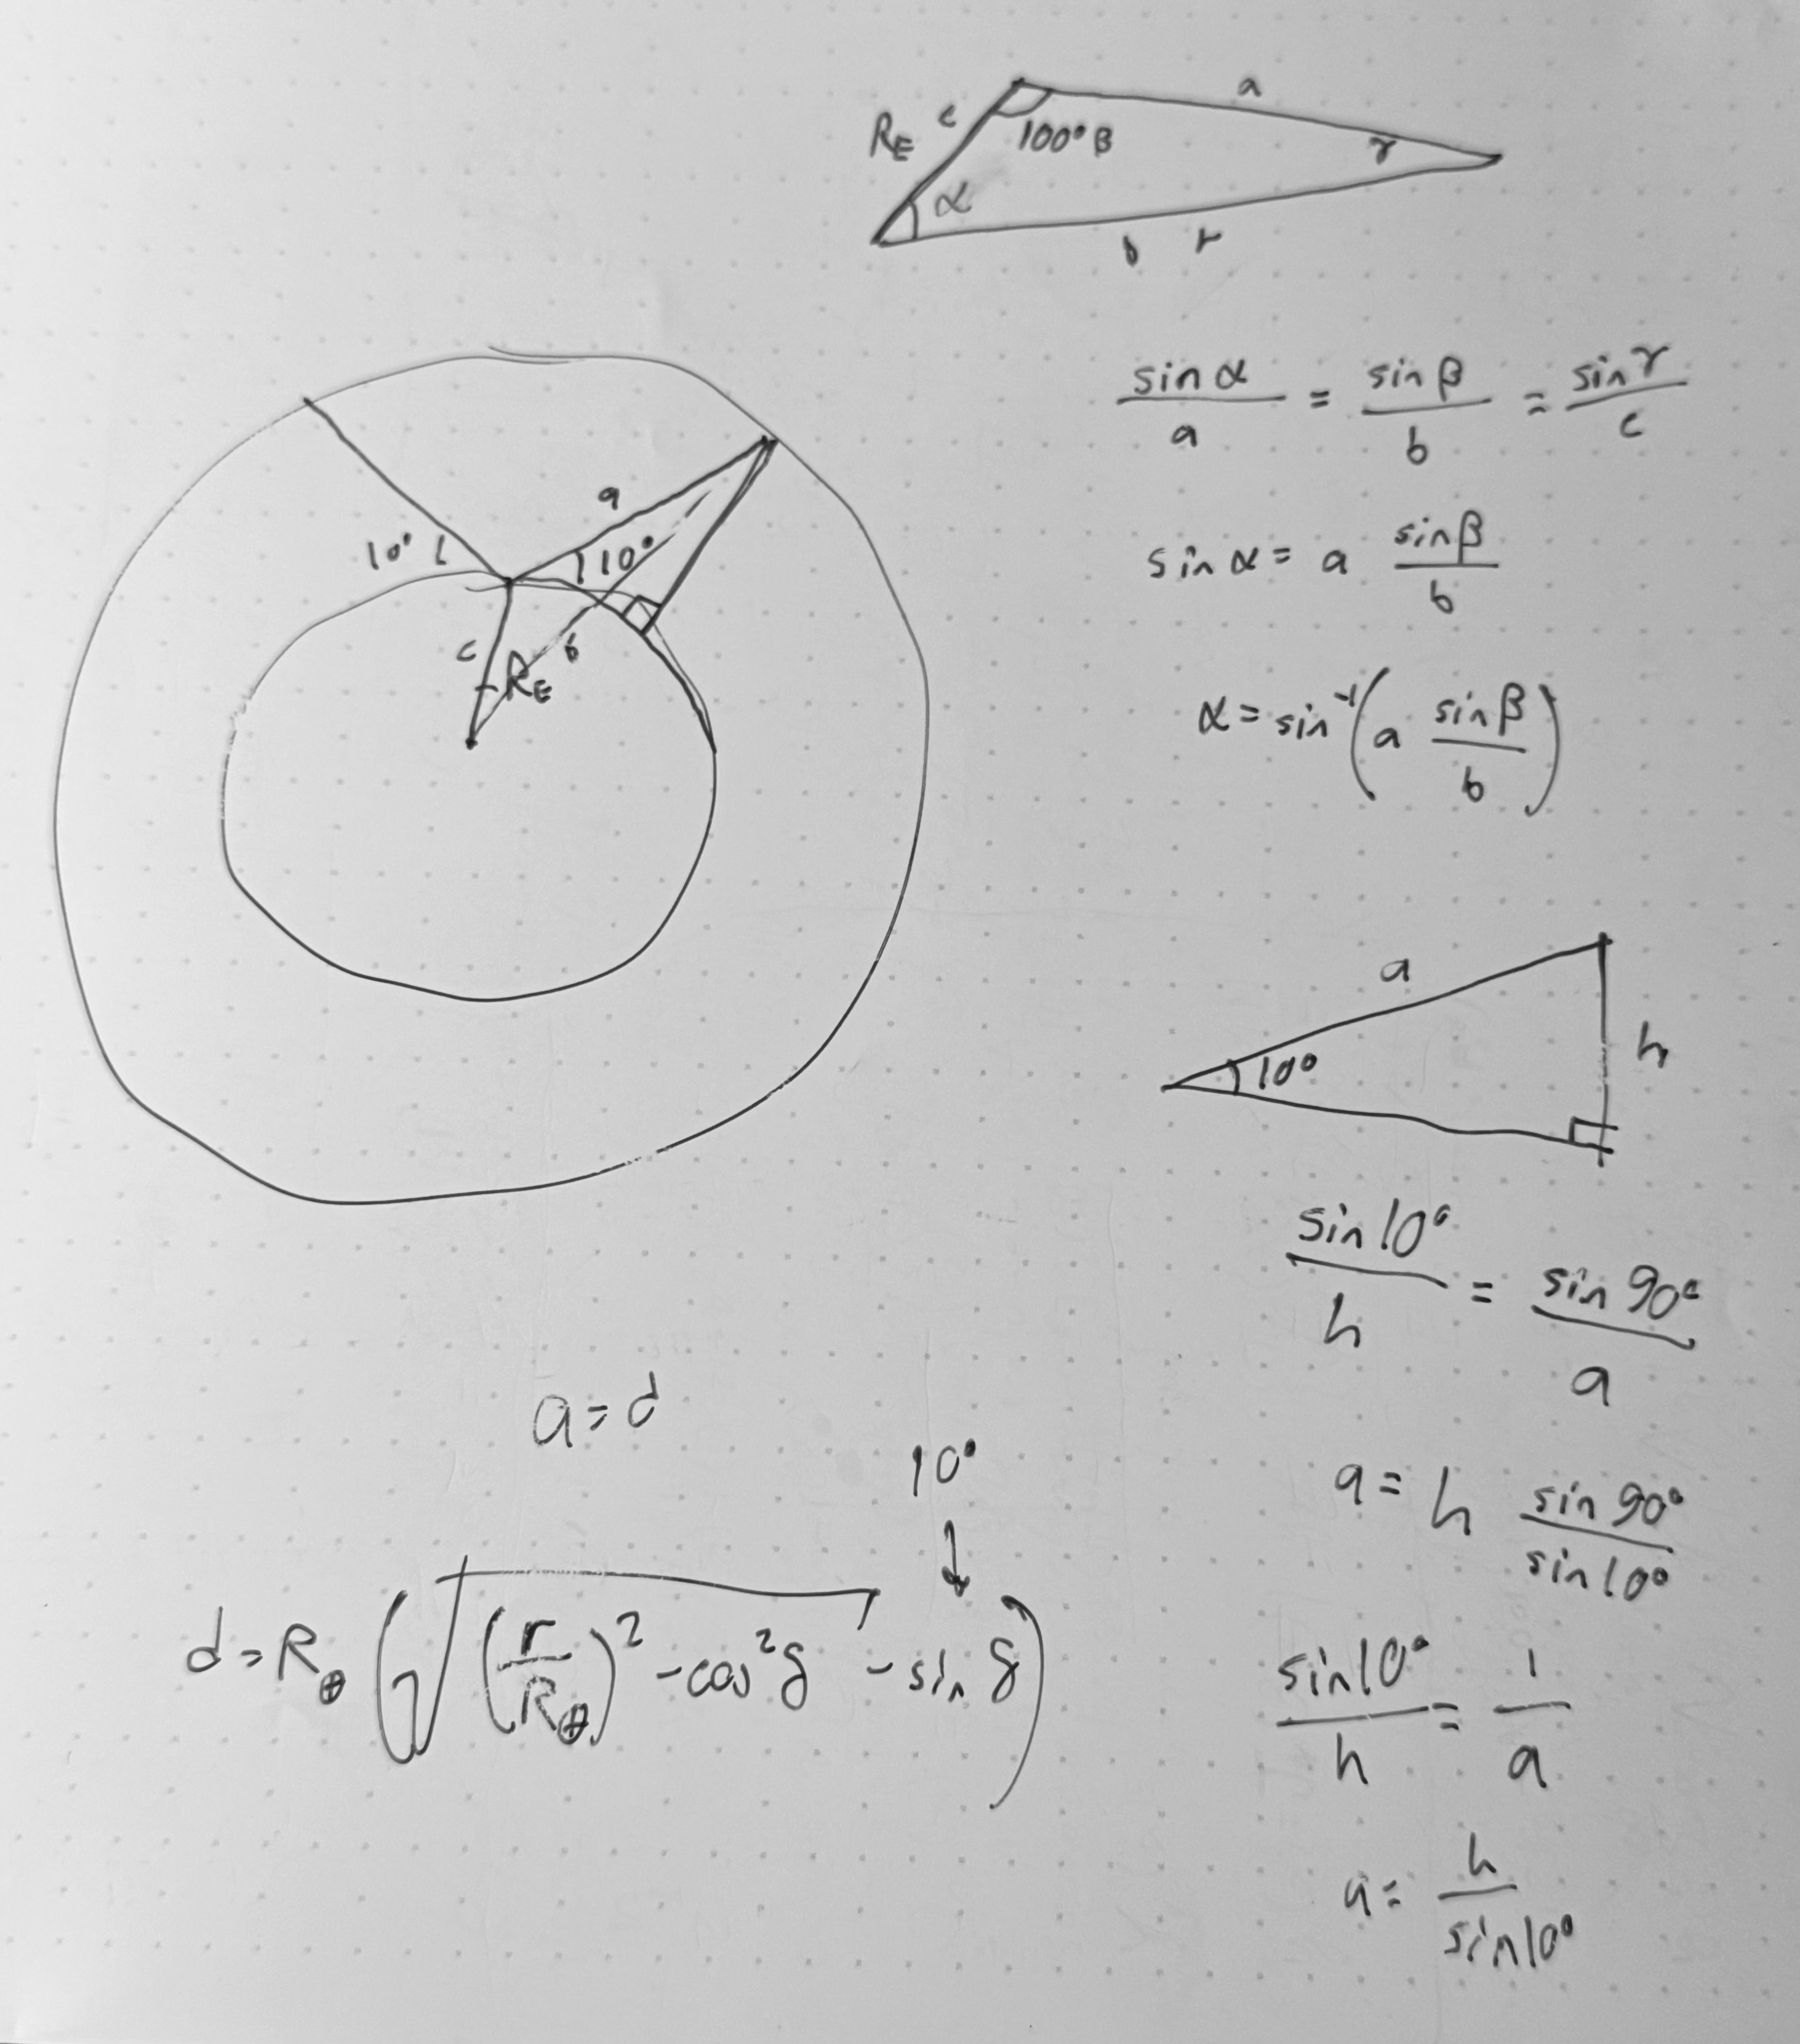
\includegraphics[width=10cm]{annulus}
  \caption{Figuring out the geometry to find the half-angle from the center of the Earth given the radius and elevation [Own work].}
  \label{fig:annulus}
\end{figure}

This makes a lot of sense -- SARGE is far away, the elevation angle of \ang{10} is pretty generous, and the groundtrack passes fairly close to Gatineau station (on a global scale, at least).

\subsection{Fun Orbital Plane Geometry}\label{app:orbplanes}

To find $\alpha$ and $\gamma$ for the orbital perturbation estimations in Appendix~\ref{app:orbpert}, I estimated the angles between SARGE's orbital plane and the Sun and the Moon using the Ecliptic plane and Lunar orbit inclination values found in a figure (with no listed author) from Wikipedia.

\begin{figure}[hb]
  \centering
  \captionsetup{width=.75\linewidth,font={small},labelfont={bf}}
  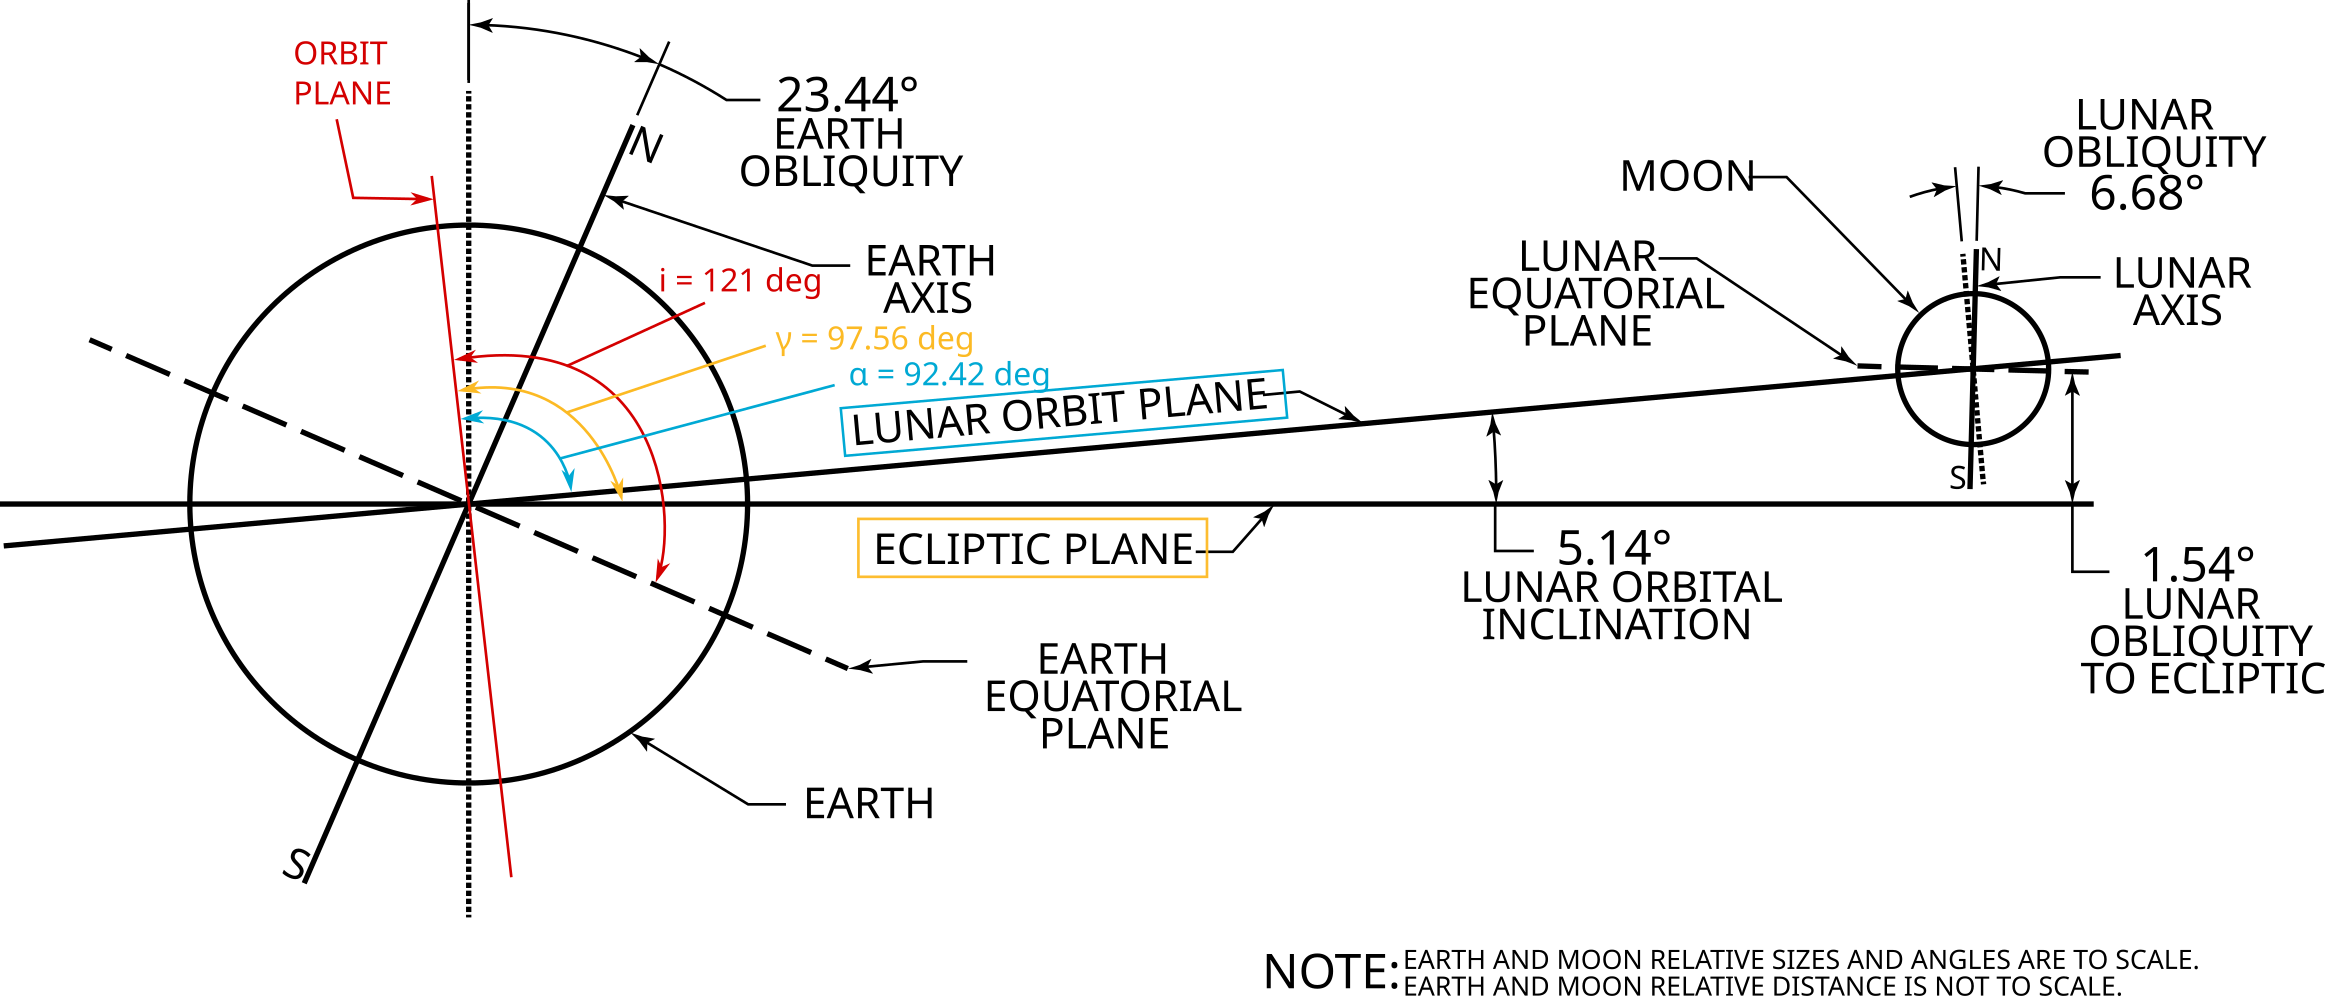
\includegraphics[width=15cm]{Annotated_Moon_Orbit}
  \caption{Angles between the orbit plane of SARGE and the Lunar orbit plane ($\alpha$) and the Ecliptic plane ($\gamma$). [Author unknown, \texttt{CC0}, annotations (in colour) added]}
  \label{fig:moonorbit}
\end{figure}

From Figure~\ref{fig:moonorbit}, we can estimate that the angle between SARGE's orbit plane and the Ecliptic plane ($\gamma$) to be \ang{97.56}, and between SARGE's orbit plane and the Lunar orbit plane ($\alpha$) as \ang{92.42}.

\section{Link Budget}\label{app:linkbudget}
\subsection{Down}
The initial step of developing the link budget is to determine how much payload data we need to download.
The area of Canada proper, shown in red in Figure~\ref{fig:groundtrack}, is about \qty{8.342e6}{\kilo\meter\squared}.
From the mission requirements, we need to image that entire area (at least) once every \qty{14}{\day}.
Assuming that the payload is capable of steering its beam in order to cover swaths of \qty{100}{\kilo\meter} width, and considering an image to be $\qty{100}{\kilo\meter}\times\qty{100}{\kilo\meter}$, with a linear resolution of \qty{5}{\meter} such that each pixel is $\qty{25}{\meter\squared}$ and contains \qty{16}{\bit} of data, we estimate the amount of data required to image all of Canada using the following:
\begin{equation}
  \text{Image Pixels} = \frac{\text{Image Area}}{(\text{Linear Resolution})^2}=\qty{4.0e8}{pixels}
\end{equation}
Then, the size of each image:
\begin{equation}
  \text{Image Size} = \text{Pixel Size}\times\text{Image Pixels} = \qty{800}{\mega\byte}
\end{equation}
Then, the images required to cover Canada, with a 4\% swath overlap accomodation:
\begin{equation}
  \text{Images per Canada} = \frac{A_\text{Canada}}{\text{Image Area}}\times 1.04 \approx \qty{868}{images}
\end{equation}
And thus, the amount of data required to image Canada once:
\begin{equation}
  \text{Canada Size} = \text{Images per Canada} \times \text{Image Size} = \qty{694.05}{\giga\byte}
\end{equation}
Over \qty{14}{\day}, the average payload data rate is then:
\begin{equation}
  R_\text{payload,avg} = \frac{\text{Canada Size}}{\qty{14}{\day}}=\qty{573.78}{\kilo\byte\per\second}
\end{equation}

This does not include the housekeeping data specified in the mission requirements and summarized in Table~\ref{tab:housekeepingdata} below.
\begin{table}[hb]
  \centering
  \captionsetup{width=.75\linewidth,font=small,labelfont=bf}
  \begin{tabular}{c|rl}
    \toprule
    Data & Quantity & Unit\\
    \midrule
    Error Detection & \num{3} & \si{\bit\per\byte}\\
    Latitude & \num{32} & \si{\bit\per image}\\
    Longitude & \num{32} & \si{\bit\per image}\\
    Altitude & \num{32} & \si{\bit\per image}\\
    Time & \num{64} & \si{\bit\per image}\\
    Synchronization & \num{24} & \si{\bit\per image}\\
    Health Data Rate & \num{26.66}\dots & \si{\bit\per\second}\\
    \bottomrule
  \end{tabular}
  \caption{Summary of required housekeeping data per mission requirements.}
  \label{tab:housekeepingdata}
\end{table}

\noindent The total housekeeping data per image can then be found via
\begin{multline}
  \text{Housekeeping per Image} = \text{Image Size}\times\text{Error Detection}+\text{Latitude}+\text{Longitude}\\+\text{Altitude}+\text{Time}+\text{Synchronization} = \qty{300}{\mega\byte\per image}
\end{multline}
The total housekeeping data per Canada:
\begin{equation}
  \text{Housekeeping Size} = \text{Housekeeping per Image} \times \text{Images per Canada} = \qty{260.27}{\giga\byte}
\end{equation}
And the average housekeeping data rate:
\begin{equation}
  R_\text{housekeeping,avg} = \frac{\text{Housekeeping Size}}{\qty{14}{\day}}+\text{Health Data Rate}=\qty{215.17}{\kilo\byte\per\second}
\end{equation}
To penultimately culminate in the \textit{average} downlink data rate:
\begin{equation}\label{eq:avgdownlinkdatarate}
  R_\text{DL,avg}=R_\text{payload,avg}+R_\text{housekeeping,avg}=\qty{788.95}{\kilo\byte\per\second}
\end{equation}
And as found in Appendix~\ref{app:annulus}, the proportion of time SARGE is within \ang{10} elevation of Gatineau is \qty{39.69}{\percent}, and thus the total access time is:
\begin{equation}\label{eq:totalaccess}
  T_\text{access} = P\times\qty{39.69}{\percent}\approx\qty{9.5}{\hour\per\day}
\end{equation}
From the guidance given in class, approximately \qty{20}{\percent} of access window should be allocated to uplink, thus the downlink window is \qty{80}{\percent} of $T_\text{access}$, and the actual downlink rate can be found:
\begin{equation}
  R_\text{DL} = \frac{R_\text{DL,avg}}{\frac{\qty{80}{\percent}\times T_\text{access}}{P}}=\qty{2.485}{\mega\byte\per\second}
\end{equation}
So the downlink rate required is about \qty{2.485}{\mega\byte\per\second}, which transmits for about \qty{7.6}{\hour} every sidereal day.
The bandwidth for QPSK (our downlink encoding scheme) is:
\begin{equation}
  B=0.6R=\qty{11.928}{\mega\hertz}
  \label{eq:downlinkbw}
\end{equation}

Then, as noted in Section~\ref{sec:configuration}, the communications satellite on SARGE is a parabolic antenna with a diameter $D_t$ of \qty{0.5}{\meter}.
Assuming a transmission efficiency $\eta_t$ of \qty{50}{\percent}, and noting that the wavelength $\lambda$ of the downlink center frequency of \qty{7.275}{\giga\hertz} is \qty{4.12}{\milli\meter}, the predicted gain is
\begin{equation}\label{eq:100}
  G_t=\eta_t\left(\frac{\pi D_t}{\lambda}\right)^2=\num{726}
\end{equation}

The path loss for the downlink direction is:
\begin{equation}\label{eq:101}
  L_\text{path}=\left(\frac{4\pi d}{\lambda}\right)^2\approx\num{6.53e-21}
\end{equation}
And the pointing accuracy loss can be estimated by finding the $\theta_{\qty{3}{\decibel}}$ angle via the relationship in slide deck 6:
\begin{equation}
  \theta_{\qty{3}{\decibel}}\approx\ang{70}\frac{\lambda}{D}=\ang{5.77}
\end{equation}
and then, assuming a pointing error $\epsilon$ of \ang{1} for the spacecraft:
\begin{equation}\label{eq:302}
  [L_\text{point}]=12\left(\frac{\epsilon}{\theta_{\qty{3}{\decibel}}}\right)^2=\qty{0.361}{\decibel}
\end{equation}

And finally, to find the required carrier to noise ratio, with a minimum bit error rate ${BER}$ of \num{10e-5} for the downlink, as suggested in slide deck 6:
\begin{equation}\label{eq:102}
  {C/N}_\text{required}=\frac RB\ln\left(\frac{1}{2{BER}}\right)=\qty{14.20}{\decibel}
\end{equation}

Whew.
\subsection{Up}
The uplink analysis is much the same as the downlink analysis presented just previously, except we just assume a transmission rate of \qty{2.5}{\kilo\bit\per\second}, and we're using BFSK as recommended in slide deck 6.
As well, for lack of better information and based on the ballparks present in the SME-SMAD, we assume a transmitter power at the basestation of \qty{200}{\watt}.
From Natural Resources Canada, the diameter of the Gatineau satellite dish is \qty{13}{\meter}, and we'll assume a pointing accuracy $\epsilon$ of \ang{0.25} and still a transmit efficiency $\eta_t$ of \qty{50}{\percent}.
Then the transmitter gain is:
\begin{equation}\label{eq:200}
  G_t=\eta_t\left(\frac{\pi D_t}{\lambda}\right)^2=\num{594e3}
\end{equation}
And the path loss is slightly different because the uplink center frequency is \qty{8.00}{\giga\hertz} with a corresponding wavelength $\lambda$ of \qty{3.75}{\milli\meter}:
\begin{equation}\label{eq:203}
  L_\text{path}=\left(\frac{4\pi d}{\lambda}\right)^2\approx\num{5.40e-21}
\end{equation}
And the $\theta_{\qty{3}{\decibel}}$:
\begin{equation}
  \theta_{\qty{3}{\decibel}}\approx\ang{70}\frac{\lambda}{D}=\ang{0.20}
\end{equation}
With a pointing loss of:
\begin{equation}\label{eq:303}
  [L_\text{point}]=12\left(\frac{\epsilon}{\theta_{\qty{3}{\decibel}}}\right)^2=\qty{18.42}{\decibel}
\end{equation}
A bandwidth of (according to slide deck 6):
\begin{align}
  B =2R(1+\beta)&=\qty{5016}{\hertz}\\\label{eq:201}
  \beta =\Delta f/f_{mod}&=\num{0.003125}\\
  \Delta f&=\qty{25}{\mega\hertz}\qquad(\text{Half of max channel BW})
\end{align}

And finally, the minimum carrier to noise is calculated in the same was as Eq.~\ref{eq:102}, but with a ${BER}$ of \num{10e-7} for telecommand, also as mentioned in slide deck 6:
\begin{equation}\label{eq:202}
  {C/N}_\text{required}=\frac RB\ln\left(\frac{1}{2{BER}}\right)=\qty{8.16}{\decibel}
\end{equation}



\vfill
\section{Preliminary Drawings}\label{app:julia}


\end{document}
